\thislesson{23 Gennaio 2017}{Biliardi ellittici e Supercazzole immaginarie}

\section{Biliardi ellittici}
\newthought{Introduciamo un altro modo} in cui si ottengono le curve
ellittiche dalle ellissi \notamargine{Abbiamo infatti già visto che si
  possono ottenere come integrali della lunghezza d'arco di un'ellisse}.

Prendiamo un'ellisse di equazione $ax^2 + by^2 = 1$ e supponiamo di
giocare a biliardo sull'ellisse: facendo partire la pallina da un punto
la lanciamo contro il bordo dell'ellisse su cui rimbalza secondo la nota
legge della riflessione \notamargine{Ovvero rispetto alla tangente
  all'ellisse nel punto rimbalza via con lo stesso angolo, come indicato
  in figura}

\begin{center}
  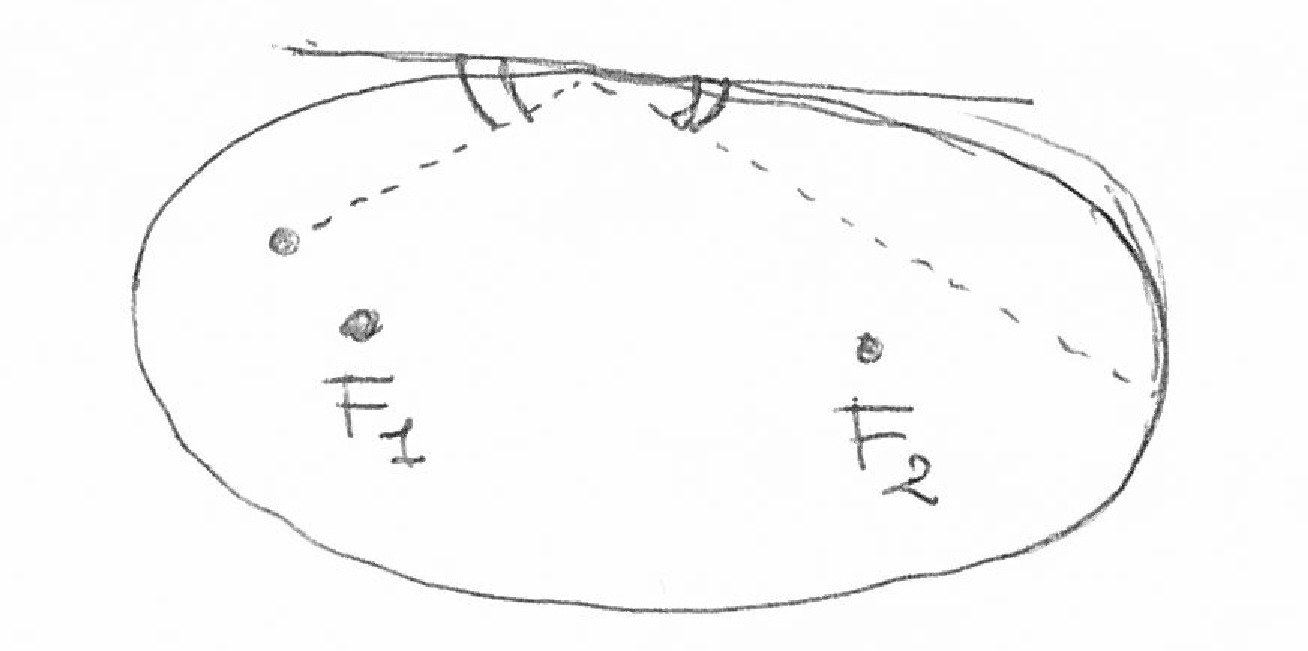
\includegraphics[width=8cm]{lezione-170123-fig1}
\end{center}
  
Una cosa che è nota da tempo è che le rette che compongono la
traiettoria sono tutte tangenti ad un'altra ellisse ``caustica'' che ha
gli stessi fuochi della prima: abbiamo quindi una famiglia ad un
parametro di ellissi che descrive tutte le possibili traiettorie.

\newthought{Vediamo allora che succede} quando prendiamo un punto $P$
sul bordo dell'ellisse ed una retta $l$ con $P \in l$ e tangente alla
caustica:

Possiamo definire un'applicazione $\phi$ dalle coppie punto-retta in sè
che è la funzione di ``evoluzione'' della traiettoria sul biliardo,
ovvero manda la coppia $(P, l)$ in $(P', l')$ con $P'$ l'altro punto di
intersezione della retta $l$ con l'ellisse e $l'$ la retta passante per
$P'$ che segue la legge della riflessione con $l$.

\notamargine{
  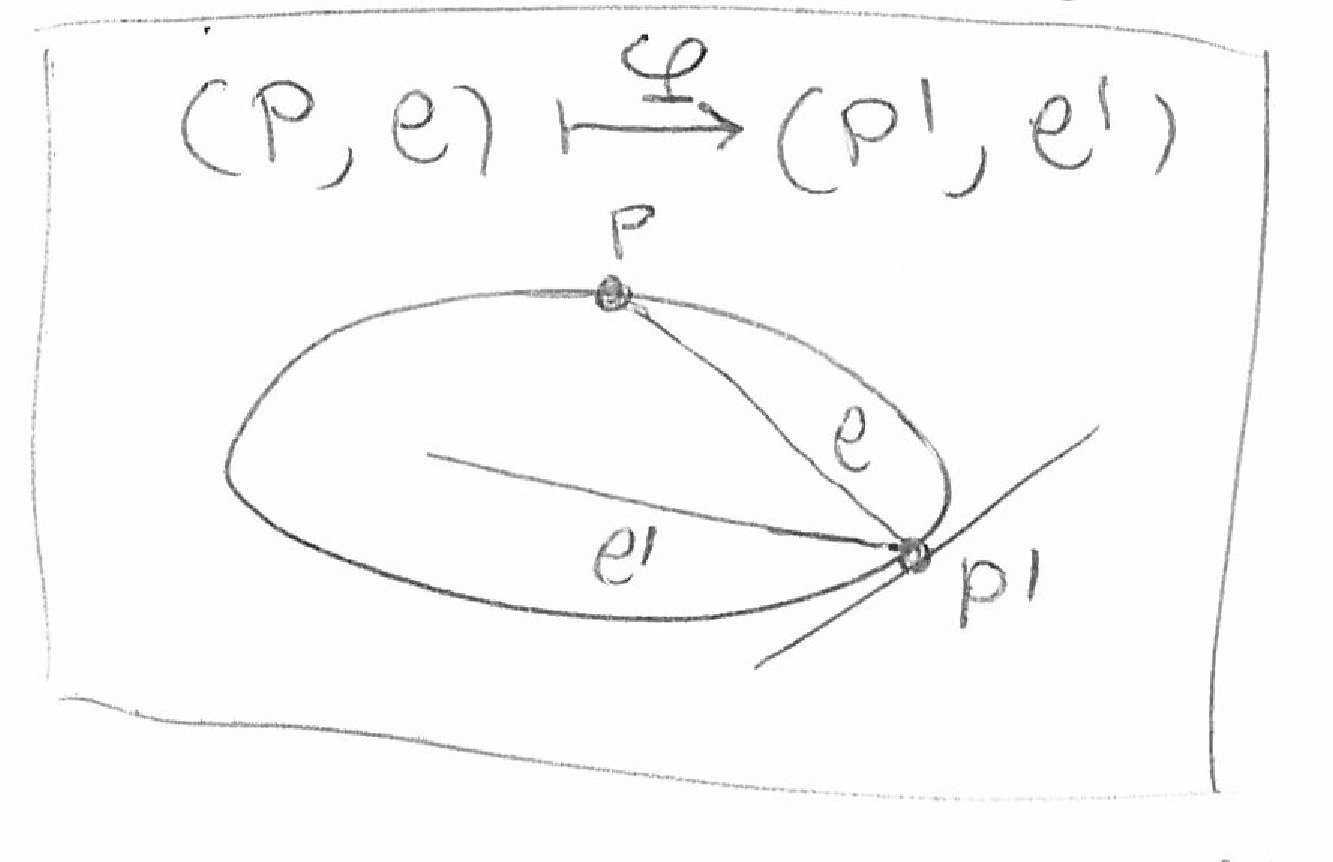
\includegraphics[width=4cm]{lezione-170123-fig2}
}

\newthought{È noto} che le tangenti in $\bbP^2$ ad una conica sono
parametrizzate da un'altra conica: la conica duale.
\notamargine{Tutto ciò non è difficile da verificare: se la conica $\cC$
  ha equazione $f = ax^2 + by^2 + cz^2$ e $(x_0, y_0, z_0) = P \in \cC$
  allora $(\nabla f)_P = (2ax_0, 2by_0, 2cz_0)$ e, ricordando che tutti
  i punti/vettori considerati sono in $\bbP^2$ si ha che dare la retta
  tangente in $P$ è uguale a fornire il vettore $(\nabla f)_P$. D'altra
  parte si riesce ovviamente a recuperare il punto $P$ dato $(\nabla
  f)_P$ a cui è tangente (basta vedere la formula scritta sopra in
  coordinate, visto che i coefficienti della conica sono noti)}
Allora il luogo di punti su cui la $\phi$ agisce è una sottovarietà
(algebrica) di $C_1 \times \hat{C_2}$, con $C_1 = \text{punti della
  conica}$ e $\hat{C_2} = \text{conica duale delle rette tangenti}$.

Il luogo di punti è dato dalle coppie $(P, l) \in C_1 \times \hat{C_2}$
tali che $P \in l$ (che è una condizione chiusa, ovvero dà luogo ad una
sottovarietà algebrica). Questa è anche una superficie di Riemann.

Scrivendo l'equazione si ottiene una curva ellittica e l'operazione
$\phi$ si rivela essere una traslazione sulla cubica detta ``gioco di
Poncelèt''.

Il gioco ``finisce'' se e solo se la traslazione $\phi(x) = x + \tau$ ha
un punto di ordine finito, ovvero $\exists n$
$\phi^n (x) = x + n\tau = x$ se e solo se $n\tau \in L$, il
reticolo. Ovvero si avrebbe $\phi^n(x) = x$ per ogni punto. Allora se il
gioco finisce per una traiettoria finisce per tutte le altre, cosa che
non è per nulla banale.

\notamargine{Come curiosità, se il gioco non finisce, le traiettorie del
  biliardo sono dense nello spazio tra le due ellissi}

\section{Funzioni Modulari}

\notamargine{Il nome ``modulari'' è riferito ai moduli, parametri che
  comparivano negli integrali ellittici. Oggi ci si riferisce a moduli
  per indicare uno spazio di parametri per una famiglia di curve
  algebriche.

  Esempio ``stupido'': $y - a x^2 = 0$ al variare di $a \in \bbC$ sono
  una famiglia di parabole (o per $a=0$ una retta). In questo caso lo
  spazio dei parametri è $\bbC$ (nel quale $a$ può variare)}

\begin{osservazione}
  Ricordiamo che conosciamo già un parametro delle cubiche:
  $j$. Infatti, se la cubica viene da un toro allora è della forma
  $y^2 = 4 x^3 - g_2 x - g_3$ e sappiamo che
  $j = 1728 \frac{g_2^3}{g_2^3 - 27 g_3^2}$ è un'invariante per
  trasformazioni proiettive delle cubiche.
\end{osservazione}

Siamo allora autorizzati a riscalare il reticolo $L$ pur restando nella
stessa classe di isomorfismo delle cubiche. Possiamo quindi supporre che
$L = \bbZ \tau + \bbZ 1$ con $\tau \in \cH = \{ z \in \bbC | \Img \tau >
0 \}$. In questo modo $g_2 = 60 \sum_{\omega \in L^*} \omega^{-4}$ e
$g_3 = 140 \sum_{\omega \in L^*} \omega^{-6}$ diventano funzioni
olomorfe di $\tau$ come parametro nel semipiano superiore e quindi pure
$j$ è una funzione di $\tau$

\begin{osservazione} \label{170123-j_suriettiva}
  Se vedessimo che $j$ assume tutti i valori in $\bbC$ ciò dimostrerebbe
  che tutte le cubiche provengono da un toro, poiché sappiamo già che
  due cubiche sono affinemente equivalenti se e solo se hanno lo stesso $j$.
\end{osservazione}

\begin{divagazione}
  Si può dimostrare che se $\tau$ è immaginario quadratico su $\bbQ$ allora
  $j(\tau)$ è un numero algebrico. Di seguito diamo una supercazzola della dimostrazione
  \notamargine{Immaginario quadratico vuol dire che soddisfa
    un'equazione di secondo grado a coefficienti in $\bbQ$, ovvero $x$ è
    tale che $\exists b, c \in \bbQ$ con $x^2 + bx + c = 0$ e che è un
    numero immaginario puro}

  Quando $\tau$ è un immaginario quadratico il reticolo ha infatti degli
  endomorfismi non banali. Se $j$ fosse trascendente, visto che gli
  endomorfismi sono funzioni razionali delle coordinate e avremmo
  $\bbQ(j, \text{funz.raz.})$ come campo finitamente generato su $\bbQ$,
  che ha grado di trascendenza uno.

  Allora si può ``specializzare'' $j$, visto che il campo è isomorfo ad
  una cosa con una variabile.

  \notamargine{Qui intendiamo ad esempio che $\bbQ(j, \sqrt{j + 2})
    \cong \bbQ(t, \sqrt{t + 2})$ con $t$ come variabile e quindi $\cong
    \bbQ(t_0, \sqrt{t_0 + 2})$ con $t_0$ trascendente.}
  
  Specializzandolo ad ogni altro numero trascendente ottengo un campo
  isomorfo e quindi tutte le curve ellittiche avrebbero degli
  automorfismi non banali (poiché hanno uguali campi) e ciò è
  impossibile poiché le cubiche con automorfismi sono in numero
  numerabile.
\end{divagazione}

Il reticolo $L$ può avere altre basi, date dall'applicazione di matrici
$\kM_{2 \times 2} (\bbZ)$ invertibili. Possiamo scegliere l'ordine dei
due elementi della base in modo da avere soltanto le matrici con
determinante uno.

Diciamo che due reticoli $\bbZ + \bbZ \tau = \bbZ + \bbZ \tau'$ sono
equivalenti se $\exists g \in \SL_2 \bbZ$
$\tc g\tau = \tau' = \frac{a \tau + b}{c \tau + d}$

Allora i tori complessi modulo isomorfismo sono in biggezione con $\cH$
modulo $\SL_2 \bbZ$ (in realtà l'azione si quozienta per $\{\pm 1\}$,
quindi l'azione è di $\bbP\SL_2 \bbZ$).

\section{Costruzione di un dominio fondamentale}

Vogliamo costruire un dominio fondamentale per lo spazio dei reticoli,
ovvero su cui agiranno le funzioni modulari.
\notamargine{Per dominio fondamentale intendiamo uno spazio in cui è
  presente esattamente un rappresentante per ogni reticolo. Nel nostro
  caso portiamo ogni reticolo nella forma $L = \bbZ + \bbZ \tau$}

Descriviamo innanzitutto la forma del dominio fondamentale:
$ F = \cH \cap \{ \Re z \in [ -\frac{1}{2}, \frac{1}{2} ) \} $
tolto l'insieme $\{ \abs{z} < 1 \} \cup \{ \abs{z} = 1 \mid \Re z > 0 \}$

e definiamo le due applicazioni
$$ S = \lbr{\begin{array}{cc} 0 & 1 \\ -1 & 0 \\ \end{array}} $$
$$ T = \lbr{\begin{array}{cc} 1 & 1 \\ 0 & 1 \\ \end{array}} $$
tra cui si hanno le relazioni $S^2 = (TS)^3 = \Id$

\begin{center}
  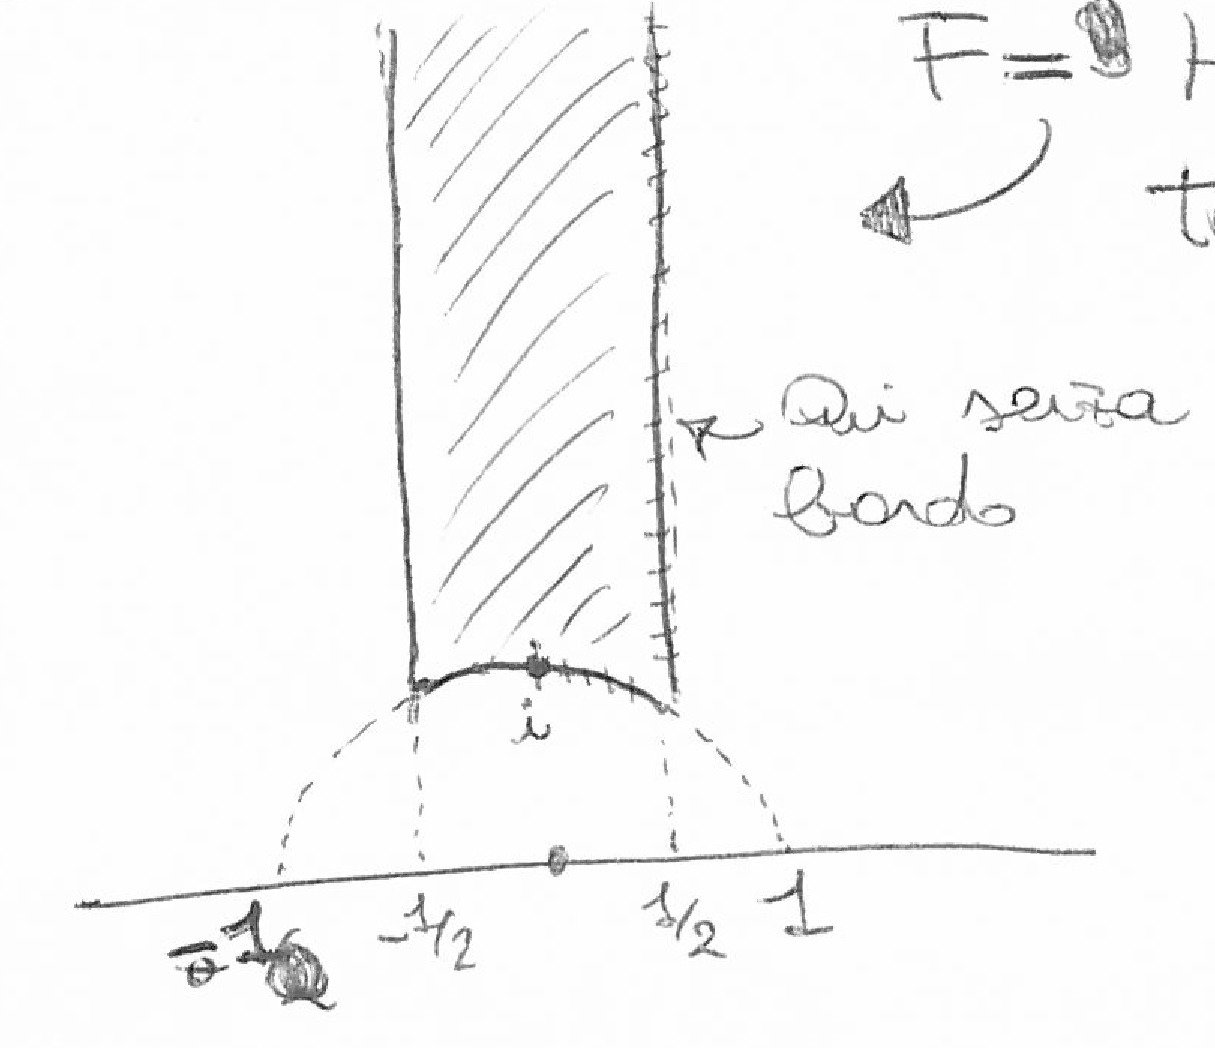
\includegraphics[width=8cm]{lezione-170123-fig3}
\end{center}

\begin{osservazione}
  Sarà parecchio importante sapere che se
  $g = \lbr{\begin{array}{cc} a & b \\ c & d \\ \end{array}} \in
  \SL_2(\bbZ)$, allora si ha $\Im (gz) = \frac{\Im z}{\abs{cz + d}^2}$.
\end{osservazione}

\begin{lemma}
  $\SL_2 \bbZ$ è un sottogruppo discreto come sottoinsieme di $\SL_2 \bbR$
  ed agisce in modo propriamente discontinuo su $\cH$
\end{lemma}
\begin{proof}
  Sia $K \subseteq \cH$ un compatto: vogliamo mostrare che allora
  $gK \cap K \neq \emptyset$ per al più un numero finito di $g \in G$.

  Allora sia $z_0 \in K$ tale che $g z_0 \in K$. Sappiamo però che per
  un qualunque compatto in $\cH$ $\exists \rho, \rho'$ che dipendono
  solo dal compatto tali che $\rho' > \Im z > \rho > 0$ per un qualunque
  $z \in K$. Se anche $g z_0 \in K$ ne segue allora che $\abs{cz_0 + d}$
  è limitato uniformemente in $z_0$ $\implies$
  $\Im (cz_0 + d) = c \Im z_0$ $\implies$ $c$ è limitato ed anche $d$ è
  limitato (e la limitazione dipende solo da $K$)

  $\frac{a z_0 + b}{c z_0 + d} \in K$. Allora, visto che le possibili
  coppie $(c, d)$ sono finite, si ha
  $a z_0 + b \in \cup_{(c, d)} (cK + d)K$ che è compatto e quindi si
  conclude come sopra (utilizzando $\rho$ e $\rho'$)
\end{proof}

Anche se l'azione è propriamente discontinua il quoziente non è comunque
rivestito perché ci sono dei punti fissi: ad esempio $Si = i$ e $ST
\zeta_3 = \zeta_3$. Ma sono gli unici due punti che danno fastidio.

\notamargine{Incollando i bordi del dominio fondamentale si può vedere
  che topologicamente lo spazio delle curve ellittiche è omeomorfo a
  $\bbC$, anche se ovviamente non può esserne biolomorfo né rivestito
  per le conseguenze del teorema di classificazione di Riemann}

Nella prossima lezione vedremo il teorema che ci mostra che $F$ come
descritto è effettivamente un dominio fondamentale e, come curiosità:
\begin{teorema}
  $G = \SL_2 \bbZ$ è generato da $S$ e da $T$. Inoltre è esattamente il
  gruppo libero su due elementi ($S$ e $T$) con le relazioni
  $S^2 = (TS)^3 = \Id$
\end{teorema}

